\part{Transforms \& Projections}
\frame{\partpage}

\begin{frame}{Recap: Vectors}
	\begin{itemize}
		\pause\item A \textbf{vector} has a \textbf{direction} and a \textbf{magnitude}, represented by its \textbf{components}:
	\end{itemize}
	\pause\begin{columns}
		\begin{column}{0.45\textwidth}
			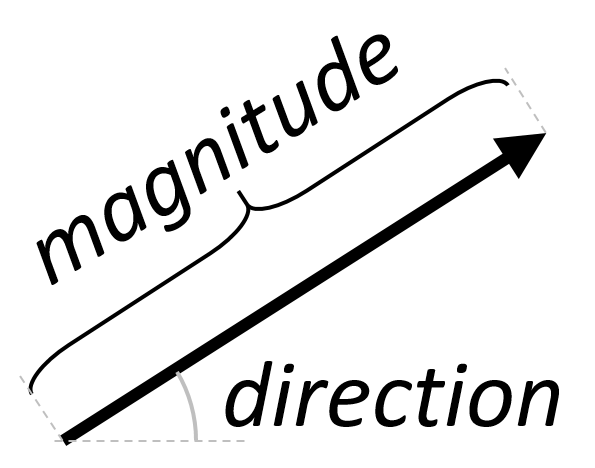
\includegraphics[width=\textwidth]{vector_polar}
		\end{column}
		\begin{column}{0.5\textwidth}
			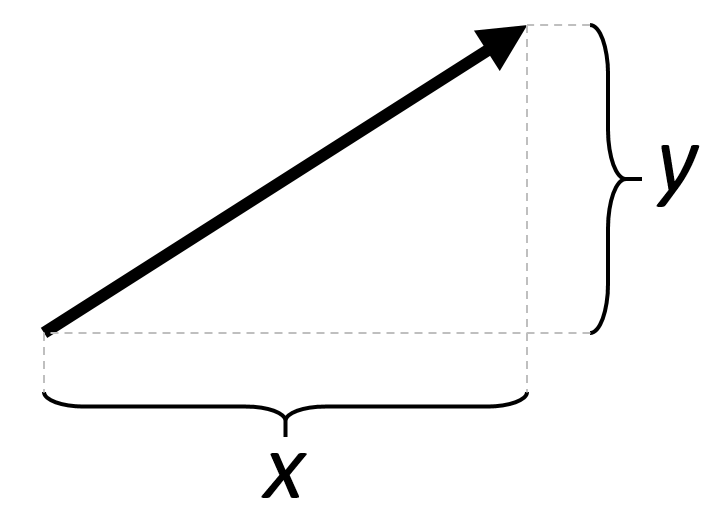
\includegraphics[width=\textwidth]{vector_components}
		\end{column}
	\end{columns}	
	\begin{itemize}
		\pause\item A vector can represent a position in space as an offset from the origin.
	\end{itemize}
\end{frame}

\begin{frame}{Recap: Matrices and Transforms}
	\begin{itemize}
		\pause\item A vector can be transformed (moved in space) by multiplying with a \textbf{matrix}:
			\begin{itemize}
				\pause\item \textbf{Translation} applies a linear offset to each component (equivalent to vector addition).
				\pause\item \textbf{Rotation} applies an angular displacement around the origin.
				\pause\item \textbf{Scale} multiplies each component by a constant (equivalent to scalar multiplication for uniform scale).
			\end{itemize}
		\pause\item Transforms can be combined by \textbf{multiplying} the matrices together.
			\begin{itemize}
				\pause\item Matrix multiplication is \textbf{NOT commutative}: the order matters.
				\pause\item Standard order is \textbf{right to left}.
				\pause\item It's generally best to apply scale first, then rotation, then finally translation - otherwise results can be unexpected...
			\end{itemize}
	\end{itemize}
\end{frame}

\begin{frame}{Recap: Coordinate Spaces}
	\begin{center}
		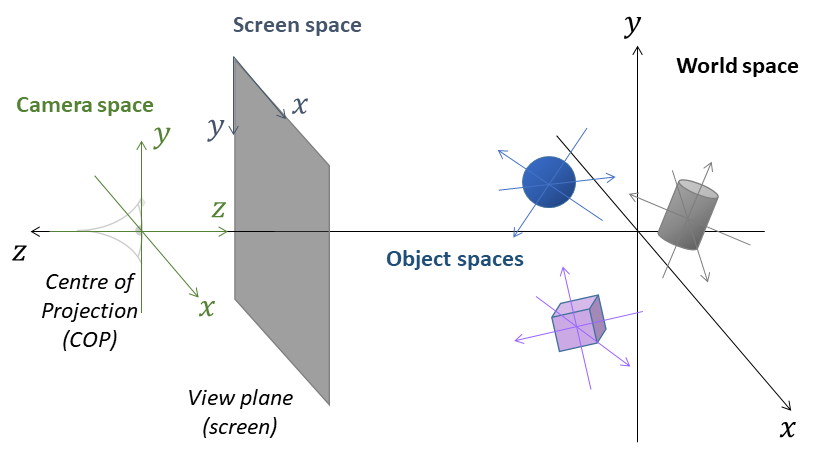
\includegraphics[width=\textwidth]{coordinate_spaces}
	\end{center}
\end{frame}

\begin{frame}{Model, View, Projection}
	\pause Drawing a 3D object on screen generally involves \textbf{three} transformations:
	\begin{itemize}
		\pause\item \textbf{Model}: translate, rotate and scale the object into its place in the scene
		\pause\item \textbf{View}: translate and rotate the scene to put the observer at the origin
		\pause\item \textbf{Projection}: convert points in 3D space to points on the 2D screen
	\end{itemize}
	\pause The \textbf{model-view-projection (MVP) matrix}:
		$$ M_{MVP} = M_{\text{projection}} \times M_{\text{view}} \times M_{\text{model}} $$
\end{frame}

\begin{frame}{The view frustum}
	\pause\begin{center}
		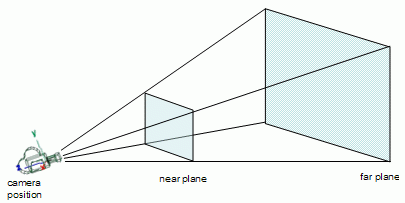
\includegraphics[width=0.8\textwidth]{frustum}
	\end{center}
	\begin{itemize}
		\pause\item Defined by the \textbf{near and far clipping planes} and the \textbf{edges of the screen}
		\pause\item \textbf{Nothing outside} the view frustum is visible
	\end{itemize}
\end{frame}


\begin{frame}{Types of projection}
	\pause\begin{center}
		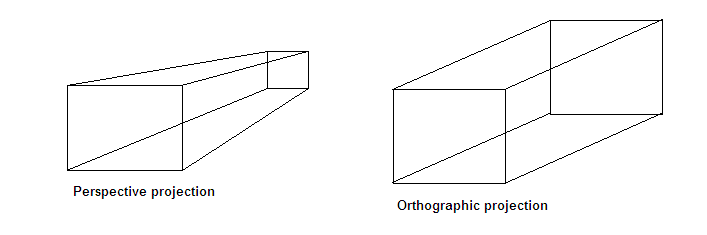
\includegraphics[width=\textwidth]{orthographic_perspective}
	\end{center}
	\begin{itemize}
		\pause\item Generally use \textbf{perspective} for 3D graphics
		\pause\item \textbf{Orthographic} is useful for 2D or pseudo-2D graphics (e.g.\ isometric projection for engineering or technical drawings)
	\end{itemize}
\end{frame}